%\documentclass[10pt,notes]{beamer}       % print frame + notes
%\documentclass[10pt, notes=only]{beamer}   % only notes
\documentclass[11pt]{beamer}              % only frames

%%%%%% IF YOU WOULD LIKE TO CREATE LECTURE NOTES COMMENT OUT THE FOlLOWING TWO LINES
%\usepackage{pgfpages}
%\setbeameroption{show notes on second screen=bottom} % Both

\usepackage{graphicx}
\DeclareGraphicsExtensions{.pdf,.png,.jpg}
\usepackage{color}
\usetheme{winslab}
\usepackage[utf8]{inputenc}
\usepackage[english]{babel}
\usepackage{amsmath}
\usepackage{amsfonts}
\usepackage{amssymb}




\usepackage{algorithm2e,algorithmicx,algpseudocode}
\algnewcommand\Input{\item[\textbf{Input:}]}%
\algnewcommand\Output{\item[\textbf{Output:}]}%
\newcommand\tab[1][1cm]{\hspace*{#1}}

\algnewcommand{\Implement}[2]{\item[\textbf{Implements:}] #1 \textbf{Instance}: #2}%
\algnewcommand{\Use}[2]{\item[\textbf{Uses:}] #1 \textbf{Instance}: #2}%
\algnewcommand{\Trigger}[1]{\Statex{\textbf{Trigger:} (#1)}}%
\algnewcommand{\Events}[1]{\item[\textbf{Events:}] #1}%
\algnewcommand{\Need}[1]{\item[\textbf{Needs:}] #1}%
\algnewcommand{\Event}[2]{\Statex \item[\textbf{On#1:}](#2) \textbf{do}}%
\algnewcommand{\Trig}[3]{\State \textbf{Trigger}  #1.#2 (#3) }%
\def\true{\textbf{T}}
\def\false{\textbf{F}}


\author[John Doe]{John Doe\\\href{mailto:john@example.com}{john@example.com}}
%\author[J.\,Doe \& J.\,Doe]
%{%
%  \texorpdfstring{
%    \begin{columns}%[onlytextwidth]
%      \column{.45\linewidth}
%      \centering
%      John Doe\\
%      \href{mailto:john@example.com}{john@example.com}
%      \column{.45\linewidth}
%      \centering
%      Jane Doe\\
%      \href{mailto:jane.doe@example.com}{jane.doe@example.com}
%    \end{columns}
%  }
%  {John Doe \& Jane Doe}
%}

\title[WINS Beamer Template]{WINS Lab Beamer Presentation Template}
\subtitle[Short SubTitle]{How to Prepare a Nice Presentation}
%\date{} 

\begin{document}

\begin{frame}[plain]
\titlepage
\note{In this talk, I will present .... Please answer the following questions:
\begin{enumerate}
\item Why are you giving presentation?
\item What is your desired outcome?
\item What does the audience already know  about your topic?
\item What are their interests?
\item What are key points?
\end{enumerate}
}
\end{frame}

\begin{frame}[label=toc]
    \frametitle{Outline of the Presentation}
    \tableofcontents[subsubsectionstyle=hide]
\note{ The possible outline of a talk can be as follows.
\begin{enumerate}
\item Outline 
\item Problem and background
\item Design and methods
\item Major findings
\item Conclusion and recommendations 
\end{enumerate} Please select meaningful section headings that represent the content rather than generic terms such as ``the problem''. Employ top-down structure: from general to more specific.
}
\end{frame}
%
%\part{This the First Part of the Presentation}
%\begin{frame}
%        \partpage
%\end{frame}
%
\section{The Problem}
%\begin{frame}
%        \sectionpage
%\end{frame}

\begin{frame}{The problem}
\framesubtitle{Tell a \alert{STORY} from the background to the conclusion}
\begin{block}{The Problem Name} 
Explain the problem here. Instead of using the term `The problem'', please use specific name for the problem. Tell us a story. Provide a picture for the scenario depicting the problem. Set the scene for average audience.
\end{block}
Spend at least \textbf{1.5-2 minutes per slide} on average.

The introduction should be something like ``I will be presenting title of talk. This is joint work with your colleagues or advisor at institution.'' 
\note{}
\end{frame}

\section{The Contribution}
\begin{frame}
\frametitle{What is the solution/contribution}
\framesubtitle{}
Explain \textbf{YOUR} contributions. Go top-down. Give the brief introduction to the contributions at the beginning of the presentation. A slide should have no more than five to six lines of text or bullets. Prefer figures instead of text: A picture is worth a thousand words.
\begin{itemize}
\item Communicate the Key Ideas
\item Don’t get Bogged Down in Details
\item Use a Top-down Approach
\end{itemize}

The audience will remember at most one single message \textbf{Which message you want to audience to remember? Can you express this message in less than a minute in an elevator?}

\end{frame}


\section{Motivation/Importance}
\begin{frame}
\frametitle{Motivation/Importance}
\framesubtitle{``Gain upon solving the problem, pain if not solved'' should be explained}
Explain why the problem is so important. Throw in a little philosophy if necessary. How does the problem fit into the larger picture? If it involves a model of a real-world phenomenon, then how good is the model? What are its applications? What makes the problem nontrivial? You can return to these issues in the Conclusion, when you can re-address them with the benefit of hindsight.
\end{frame}

\section{Background/Model/Definitions/Previous Works}


\subsection{Model, Definitions}

\frame{
\frametitle{Model, Definitions}
\framesubtitle{Formal definition of a Stochastic Process}
The use of terminology and jargon should be kept to a minimum, but is impossible to avoid entirely. All terms must be introduced early. It is also useful to remind the audience of the definitions at critical points later in the talk.

Background and this slide can be combined....
}

\subsection{Background, Previous Works}
\begin{frame}{Background}
Research is not usually carried out in a vacuum. There will almost always be other relevant or related work, which you should describe. Present an orderly synopsis of these previously- obtained results. A table is often used for this purpose. Be sure to mention the author of each paper and its date of publication. \textbf{Compare and contrast them with each other and with your paper.}
\end{frame}




\section{Contribution}
\subsection{Main Point 1}
\begin{frame}{Main Point 1: A Figure}
\framesubtitle{Abstract the Major Results}
Describe the key results of the paper. You may present the statements of the major theorems, but not their proofs. You will probably have to get a little technical here, but do so gradually and carefully.

\begin{figure}
    \centering
    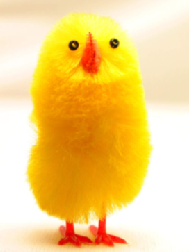
\includegraphics[scale=0.5]{figures/Chick1.png}
    \caption{Awesome Image}
    \label{fig:awesome_image}
\end{figure}
\note{
}
\end{frame}


\subsection{Main Point 2}

\begin{frame}
\frametitle{An Example Distributed Algorithm}
\framesubtitle{Blind Flooding}


Blind flooding on an undirected graph is presented in Algorithm~\ref{alg:blindflooding}.

\begin{center}
\begin{algorithm}[H]
	\scriptsize
	\def\algorithmlabel{BlindFlooding}
    \caption{\algorithmlabel\ algorithm}
    \label{alg:blindflooding}
    \begin{algorithmic}[1]
    	\Implement {\algorithmlabel}{cf} 
    	\Use {LinkLayerBroadcast} {lbc} 
    	\Events{Init, MessageFromTop, MessageFromBottom}
	\Need {}

        \Event {Init}{}
        		
        \Event{MessageFromBottom} { $m$ }
        		\Trig{lbc}{Broadcast} { $m$  }
        		
        \Event{MessageFromTop} { $m$ }	
        		\Trig{lbc}{Broadcast} { $m$  }
    \end{algorithmic}
\end{algorithm}
\end{center}


\end{frame}

\begin{frame}
\frametitle{Main Point 2}
\framesubtitle{Explain the Significance of the Results}
Pause, and explain the relationships between the formal theorems that you have just presented and the informal description that you gave in the Introduction. Make it clear to the audience that the results do live up to the advance publicity. If the statements of the theorems are very technical then this may take some time. It is time well-spent.

\end{frame}

\subsection{Main Point 3}
\begin{frame}
\frametitle{Main Point 3}
\framesubtitle{Sketch a Proof of the Crucial Results}
The emphasis is on the word ``sketch''. Give a very high-level description of the proofs, emphasizing the proof structure and the proof techniques used. If the proofs have no structure (in which case it may be assumed that you are not the author of the paper), then you must impose one on them. Gloss over the technical details. It is a good idea to point them out but not to explore them.
\end{frame}


\section{Experimental results/Proofs}

\subsection{Main Result 1}
\begin{frame}
\frametitle{Main Result 1}
\framesubtitle{}
Choose \textbf{just the key results}. They should be important, non-trivial, should give the flavour of the rest of the technical details and should be presentable in a relatively short period of time. Use figures instead of tables instead of text.

Better to present 10\% the entire audience gets than 90\% nobody gets
\end{frame}


\subsection{Main Result 2}
\begin{frame}
\frametitle{Main Result 2}
\framesubtitle{Try a subtitle}
\begin{itemize}
\item Make sure your notation is clear and consistent throughout the talk. Prepare a slide that explains the notation in detail, in case that is needed or if somebody asks.
\item Always label all of your axes on graphs; use short but helpful captions on figures and tables. It is also very useful to have an arrow on the side which clearly shows which direction is considered better (e.g., "up is better").
\item If you have experimental results, make sure you clearly present the experimental paradigm you used, and the details of your methods, including the number of trials, the specific analysis tools you applied, significance testing, etc.
\item The talk should contain at least a brief discussion of the limitations and weaknesses of the presented approach or results, in addition to their strengths. This, however, should be done in an objective manner -- don't enthusiastically put down your own work.
\end{itemize}
\end{frame}


\subsection{Main Result 3}
\begin{frame}
\frametitle{Main Result 3}
\framesubtitle{}
\begin{itemize}
\item If time allows, the results should be compared to the most related work in the field. You should at least prepare one slide with a summary of the related work, even if you do not get a chance to discuss it. This will be helpful if someone asks about it, and will demonstrate your mastery of the material.
\item Spell check again.
\item Give for each of the x-axis, y-axis, and z-axis
\item Label, unit, scale (if log scale)
\item Give the legend
\item Explain all symbols
\item Take an example to illustrate a specific point in the figure
\end{itemize}
\end{frame}



\section{Conclusions}
\begin{frame}
\frametitle{Conclusions}
\framesubtitle{Hindsight is Clearer than Foresight}
Advices come from \cite{spillman2000present}.
\begin{itemize}
\item You can now make observations that would have been confusing if they were introduced earlier. Use this opportunity to refer to statements that you have made in the previous three sections and weave them into a coherent synopsis. You will regain the attention of the non- experts, who probably didn’t follow all of the Technicalities section. Leave them feeling that they have learned something nonetheless.
\item Give Open Problems It is traditional to end with a list of open problems that arise from your paper. Mention weaknesses of your paper, possible generalizations, and indications of whether they will be fruitful or not. This way you may defuse antagonistic questions during question time.
\item Indicate that your Talk is Over
An acceptable way to do this is to say “Thank-you. Are there any questions?”\cite{einstein}
\end{itemize}

\end{frame}

\section*{References}
\begin{frame}{References}
\tiny
\bibliographystyle{IEEEtran}
\bibliography{refs}
\end{frame}

\begin{frame}{How to prepare the talk?}
Please read \url{http://larc.unt.edu/ian/pubs/speaker.pdf}
\begin{itemize}
\item The Introduction:  Define the Problem,    Motivate the Audience,    Introduce Terminology,    Discuss Earlier Work,    Emphasize the Contributions of your Paper,    Provide a Road-map.
\item The Body:    Abstract the Major Results, Explain the Significance of the Results, Sketch a Proof of the Crucial Results
\item Technicalities: Present a Key Lemma, Present it Carefully
\item The Conclusion: Hindsight is Clearer than Foresight, Give Open Problems, Indicate that your Talk is Over
\end{itemize}

\note{
\begin{itemize}
\item The Introduction:  Define the Problem,    Motivate the Audience,    Introduce Terminology,    Discuss Earlier Work,    Emphasize the Contributions of your Paper,    Provide a Road-map.
\item The Body:    Abstract the Major Results, Explain the Significance of the Results, Sketch a Proof of the Crucial Results
\item Technicalities: Present a Key Lemma, Present it Carefully
\item The Conclusion: Hindsight is Clearer than Foresight, Give Open Problems, Indicate that your Talk is Over 
\end{itemize}
}
\end{frame}



\thankslide




\end{document}